\section{Signal}
	Computer program Garfield \cite{garfield} is designed for detailed simulation of two- and three-dimensional gas detectors. So we will perform STRAW tube studies using this program.
	
	Charged particle  create electron-ion pairs wile traverse the drift tube. Electrons under affecting the electric field drift to the wire anode (see Fig.\ref{fig:track_reconstruction}). During the travel they increase their energy and invoke an avalanche. Therefore they produce a measurable signal.

	Initial electrons drift to the wire due to the electrical field between the wire and the tube wall. Electrons ionize gas molecules due to the high electric field around the wire, especially near the wire when the strength of the electric field becomes very large.  Subsequently readout electronics process the signal induced on the wire.
	  
	The event is registered if signal reach some a threshold voltage (Fig. \ref{fig:signal_example}). So the value of threshold is a key factor on the way of searching optimal setting for signal processing procedure.
	
	\begin{table}[h]
	\centering
	\caption[Table caption text]{STRAW tube parameters }
	\begin{tabular}{|l|l|p{8cm}|}
		\hline
		parameter name & value \\
		\hline
		wire & $30~\mu m$ gold-plated Tungsten\\
		\hline
		straw length & $5~m$ \\
		\hline
		voltage & $1750~V$ \\
		\hline
		inner tube radius & $9.8~mm$ \\
		\hline
		wire medium density & $19.3 ~g/cm^3$ \\
		\hline
		wire tension& $\sim 90~g$ \\
		\hline
		working tube gas mixture & $Ar~70\% ~CO_230\%$ \\
		\hline
	\end{tabular}
	
	\label{table:straw_par}
	\end{table}		
	
	We have to set threshold as low as possible but enough above from noise level to achieve best rate of true/false detected tracks and highest track registration precision and efficiency.
	
	A variation of the signal height introduces a variation in the time when the signal passes the threshold and is considered to be the main contribution to the STRAW tracker resolution. 
	
	\begin{figure}[!h]
	\centering
	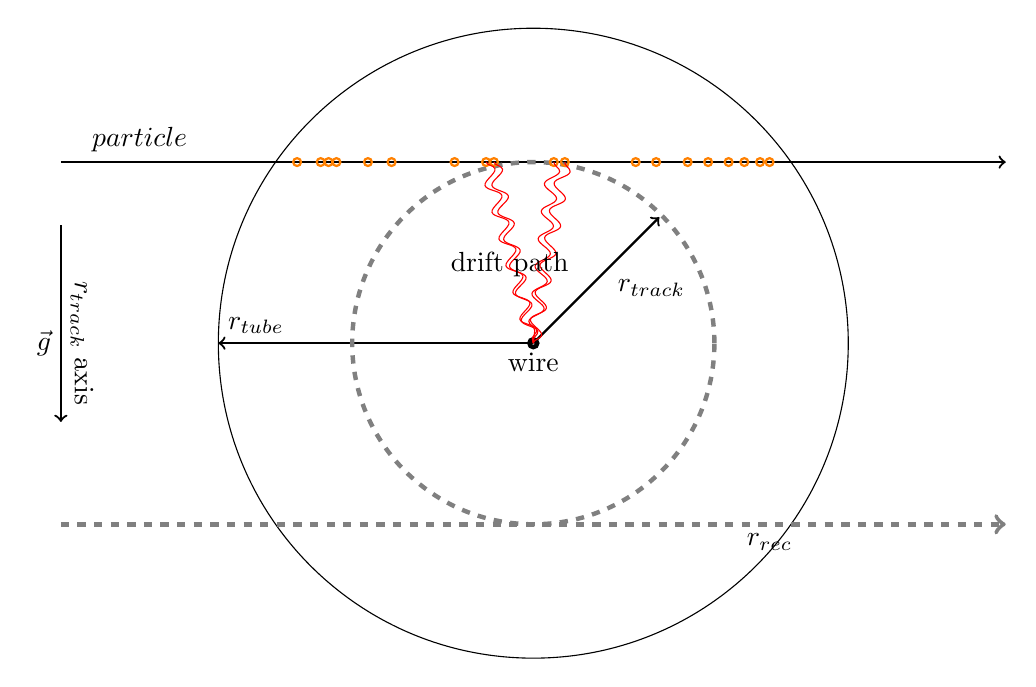
\begin{tikzpicture}
	
	\tikzset{snake it/.style={decorate, decoration=snake}}
	
	\draw (0,0) circle (4);
	
	\draw[ultra thick] (0,0) circle (0.05);
	\node[below] at (0,0) {wire};
	
	\draw[thick,->] (0,0) -- (1.6,1.6);	
	\node at (1.5,0.7) {$r_{track}$};

	\draw[thick,->] (0,0) -- (-4,0);	
	\node[above right] at (-4,0) {$r_{tube}$};
		
	\draw[thick,->] (-6,2.3) -- (6,2.3);
	\node[above] at (-5,2.3) {$particle$};
	
	\draw[ultra thick, gray, dashed, ->] (-6,-2.3) -- (6,-2.3);
	
	\draw[ultra thick,gray,dashed] (0,0) circle (2.3);
	\node[below] at (3,-2.3) { $r_{rec}$};
	
	% gravitation force vector
	\draw[thick, ->] (-6,1.5) -- ( -6, -1);
	\node[left] at (-6,0) {$\vec{g}$};
	
	% r_track axis
	\node[above,rotate=-90] at (-6,0) {$r_{track}$ axis};
	
	% initial ekectron/ion clusters
	\draw[thick,orange] (-3.0,2.3) circle(0.05);
	\draw[thick,orange] (-2.7,2.3) circle(0.05);
	\draw[thick,orange] (-2.6,2.3) circle(0.05);
	\draw[thick,orange] (-2.5,2.3) circle(0.05);
	\draw[thick,orange] (-2.1,2.3) circle(0.05);
	\draw[thick,orange] (-1.8,2.3) circle(0.05);
	\draw[thick,orange] (-1.0,2.3) circle(0.05);
	\draw[thick,orange] (-0.6,2.3) circle(0.05);
	\draw[thick,orange] (-0.5,2.3) circle(0.05);
	\draw[thick,orange] (0.26,2.3) circle(0.05);
	\draw[thick,orange] (0.4 ,2.3) circle(0.05);
	\draw[thick,orange] (1.3 ,2.3) circle(0.05);
	\draw[thick,orange] (1.56,2.3) circle(0.05);
	\draw[thick,orange] (1.96,2.3) circle(0.05);
	\draw[thick,orange] (2.22,2.3) circle(0.05);
	\draw[thick,orange] (2.48,2.3) circle(0.05);
	\draw[thick,orange] (2.68,2.3) circle(0.05);
	\draw[thick,orange] (2.88,2.3) circle(0.05);
	\draw[thick,orange] (3.00,2.3) circle(0.05);
	
	\draw[red,snake it](-0.6,2.3) -- (0,0);
	\draw[red,snake it](-0.5,2.3) -- (0,0);
	\draw[red,snake it](0.26,2.3) -- (0,0);
	\draw[red,snake it](0.4,2.3) -- (0,0);
	\node[] at (-0.3,1) {drift path};
	
	\end{tikzpicture} 
	\caption{Schematic view of a particle passing the straw and producing
ionization clusters (orange points). Electrons of ionization cluster drift to the wire and induce the signal. The closest distance from the track to the wire, $r_{track}$, and radius of the straw, $r_{tube} = 2.45 mm$, are also indicated. }
	\label{fig:track_reconstruction}
	\end{figure}


	In the track reconstruction software(GARFIELD \cite{garfield}) an effective TR-relation is used. It only describes the relation between the drift time and the distance from the track to the wire, which differs from the distance to the ionization cluster. The shape of the TR-relation is defined by the drift velocity of the ionization cluster inside the straw. The electric field increases towards the wire, leading to a non linear TR-relation. 

	The drift time versus the unbiased distance distribution and the result of the fit are shown in Fig. \ref{fig:t_r_distr_00}. Noise hits under the main distribution, i.e. at earlier times, are due to primary or secondary particles ($\delta$-rays) passing the straw at a closer distance to the wire, consequently producing an earlier signal. Initial clusters along the track are marked by orange points in the figure.
	
	Muon $\mu$ was chosen as test particle for simulation with energy $1GeV$. You can see some of typical tracks from the $\mu$ through the tube Fig.\ref{fig:electron_ion_track},\ref{fig:electron_ion_track_sag}. 
			
	
	\subsection{ Leakage noise}
	Every time we deal with different kind of noise. Basically it is noise from  leakage current through readout electronics.

	As will be discussed further we analyse not the current invoked by particle but the output voltage from amplifier. In GARFIELD we able convolute input current $I(t)$ with electronic response function (\ref{eq:responce_function}) \footnote{in this equation $t$ in nanoseconds} 
	
	\begin{equation}
	f_{resp} =  A\cdot(e^{-t/0.005} - e^{-t/0.030})
	\label{eq:responce_function}
	\end{equation}
	
	Noise is very important for every calculations and it makes bit impact on straw precision and straw efficiency. So we can't rely on results until we receive signal and noise  from real STRAW tube prototypes. 
		
	Convolution of input current makes it smooth. Usually in typical conditions\footnote{as in table \ref{table:straw_par}} noise have gauss distribution with RMS equal to a amplitude of signal from 2000 electron in the tube - electric noise charge (ENC)\footnote{With testing of real 5 m long straws and ultimate examples of electronics we will measure real noise. But for now it is only close to reality suggestion concerning to this issue.} On Fig.\ref{fig:signal_example} you can see deposition from noise marked by blue line.

	On the Fig.\ref{fig:signal_example} the timestamp $Time=0$ corresponds to the time when muon hits a tube. The convolution function smooths and spreads input current. It mean that the output voltage in GARFIELD does not contain part of signal before hit event timestamp.

	\begin{figure}[h!]
	\centering
	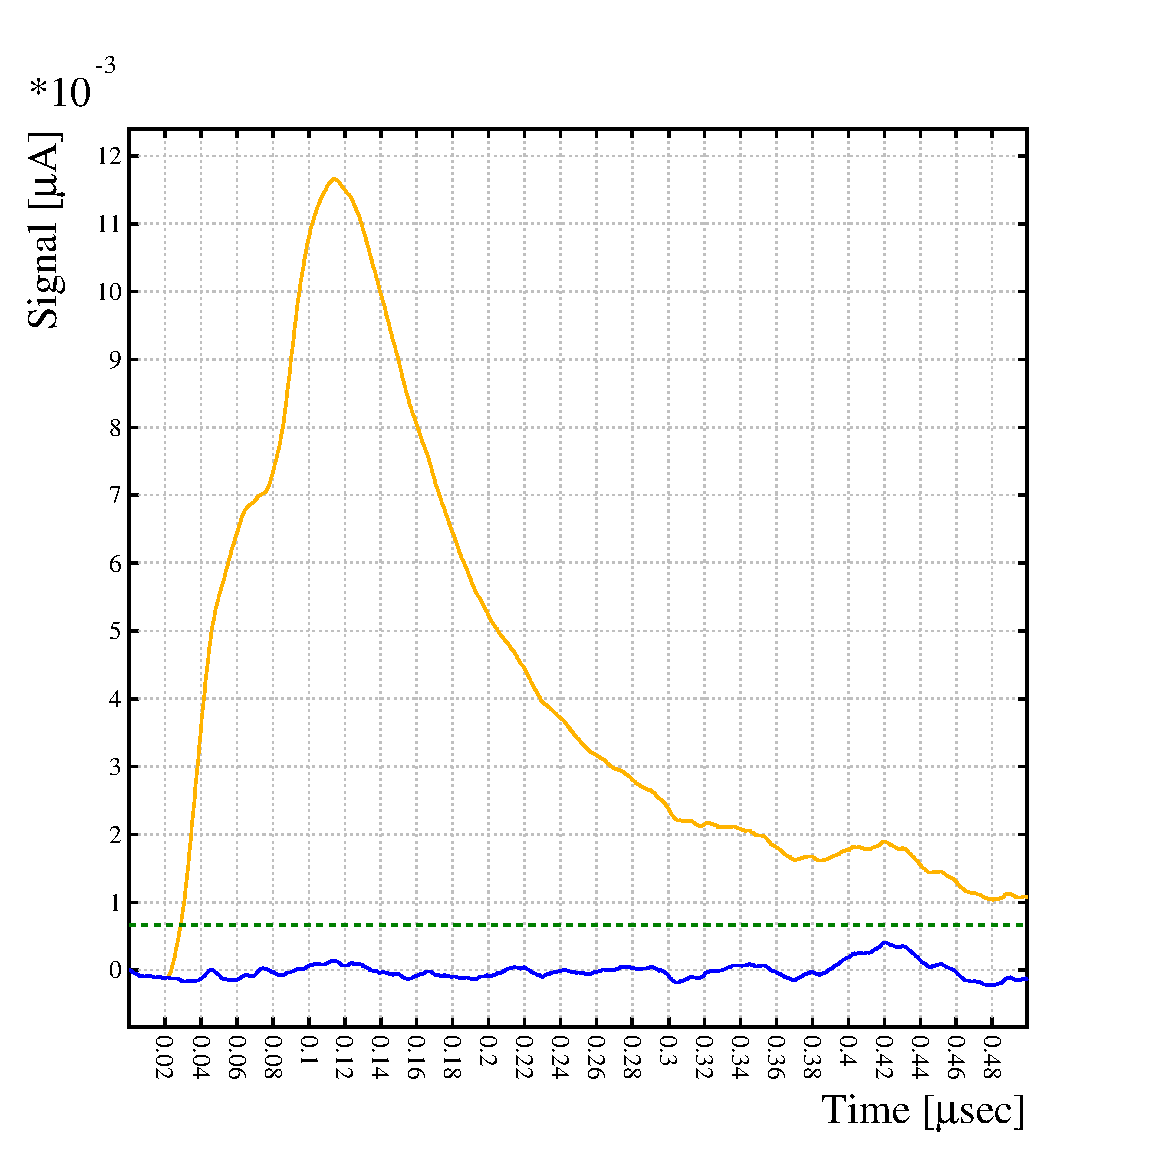
\includegraphics[width=0.7\textwidth]{signal_noise_threshold.eps}
	\caption{ Example of output signal $V(t)$ after convolution (front-end electronics) from central track (yellow line). The noise component of the same signal depicted by separate blue line. Grin dashed line is a threshold for trigering drift time and equals to $5\sigma$ of noise distribution.}
	\label{fig:signal_example}
	\end{figure}
	
	\subsection{ STRAW efficiency}
	
	The interaction of charge particle with gas molecules has probabilistic nature. For short distance tracks (somewhere near the tube wall) the probability of tracks that generation of zero electron/ion pairs becomes significantly high.
	
	The number of produced ionization clusters directly affects the hit efficiency profile. Smaller ionization length increases the hitting efficiency because of production more ionization clusters per length unit \cite{kozlinskiy}. In GARFIELD we can easily calculate amount of clusters per track. In Fig.\ref{fig:cluster_distrib} you can see a distribution of number of clusters per central track for our STRAW tube. It means that straw efficiency will be lower near the tube wall (see Fig.\ref{fig:efficiency}).
		

	\begin{figure}[h!]
	\centering
	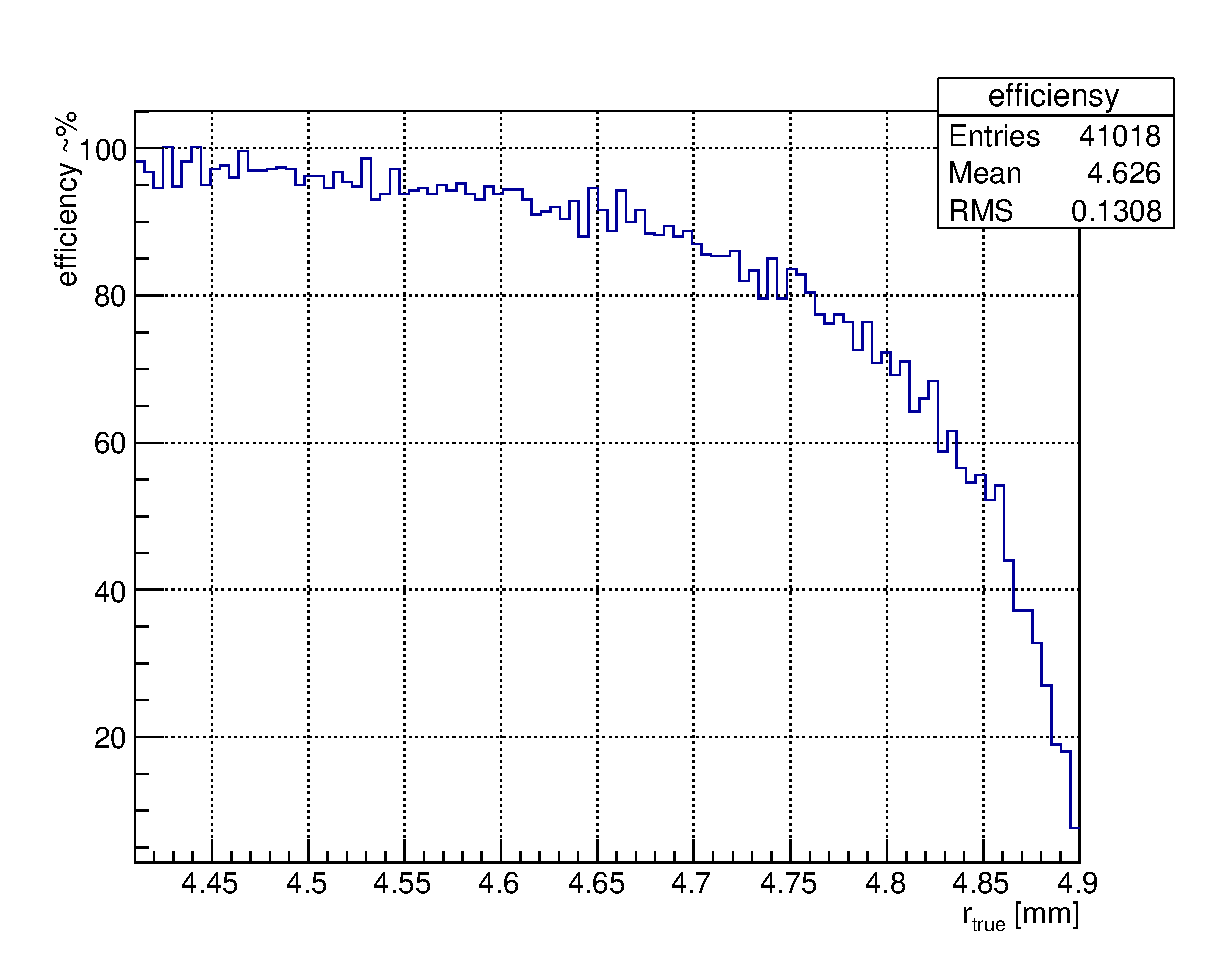
\includegraphics[width=0.8\textwidth]{periffEff}
	
	\caption{Straw tube efficiency. Result of homogeneous penetrating periphery of tube by 50k events (scaled down by factor of 5. $\dfrac{50k~events}{100 bin}  = 500 \dfrac{eventst}{bin}$).}
%	Ефективність реєстрації треків в області периферії трубки від рівномірного опромінення 50 тис. треків
	\label{fig:efficiency}
	\end{figure}	
	
	\begin{figure}[h!]
		\centering
		\subfloat[electrons per cluster]{
			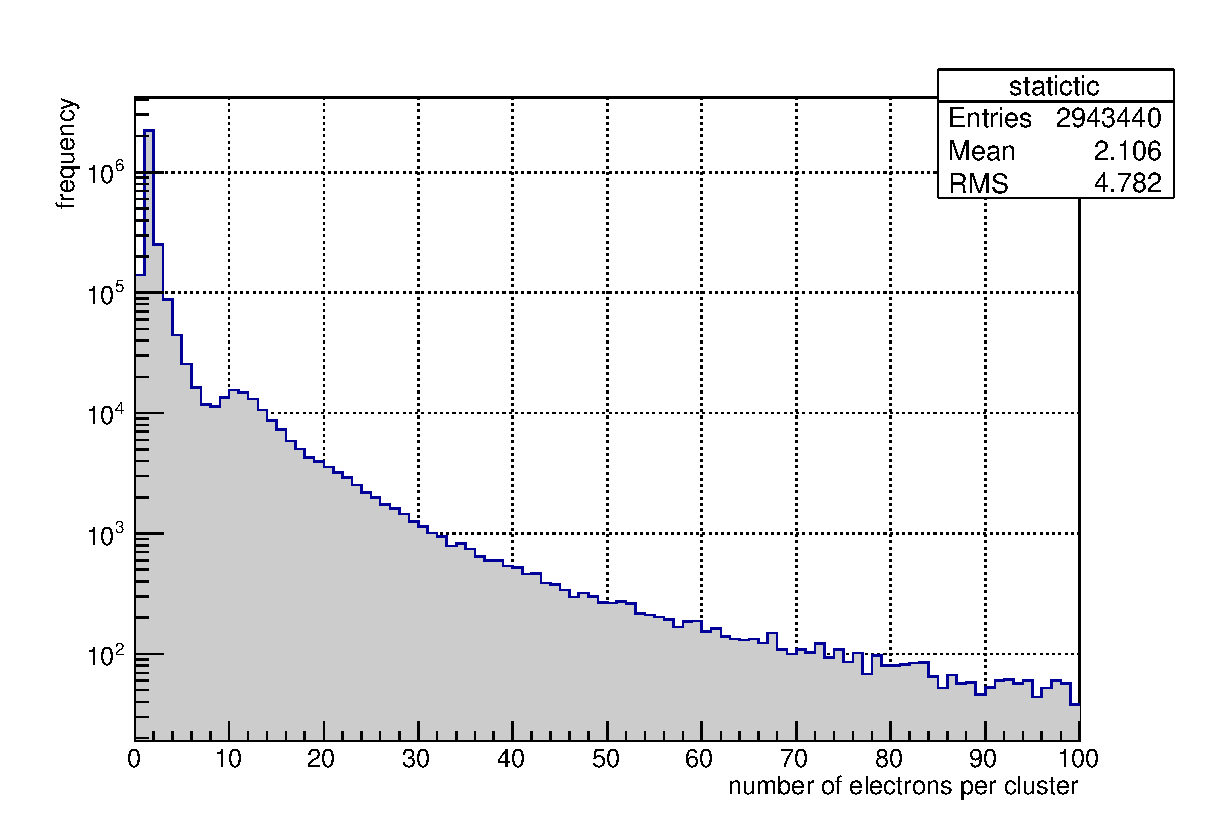
\includegraphics[width=0.45\textwidth]{el_per_cluster} 
			\label{fig:el_per_cluster} }%
		\qquad
		\subfloat[number of clusters per central track]{
			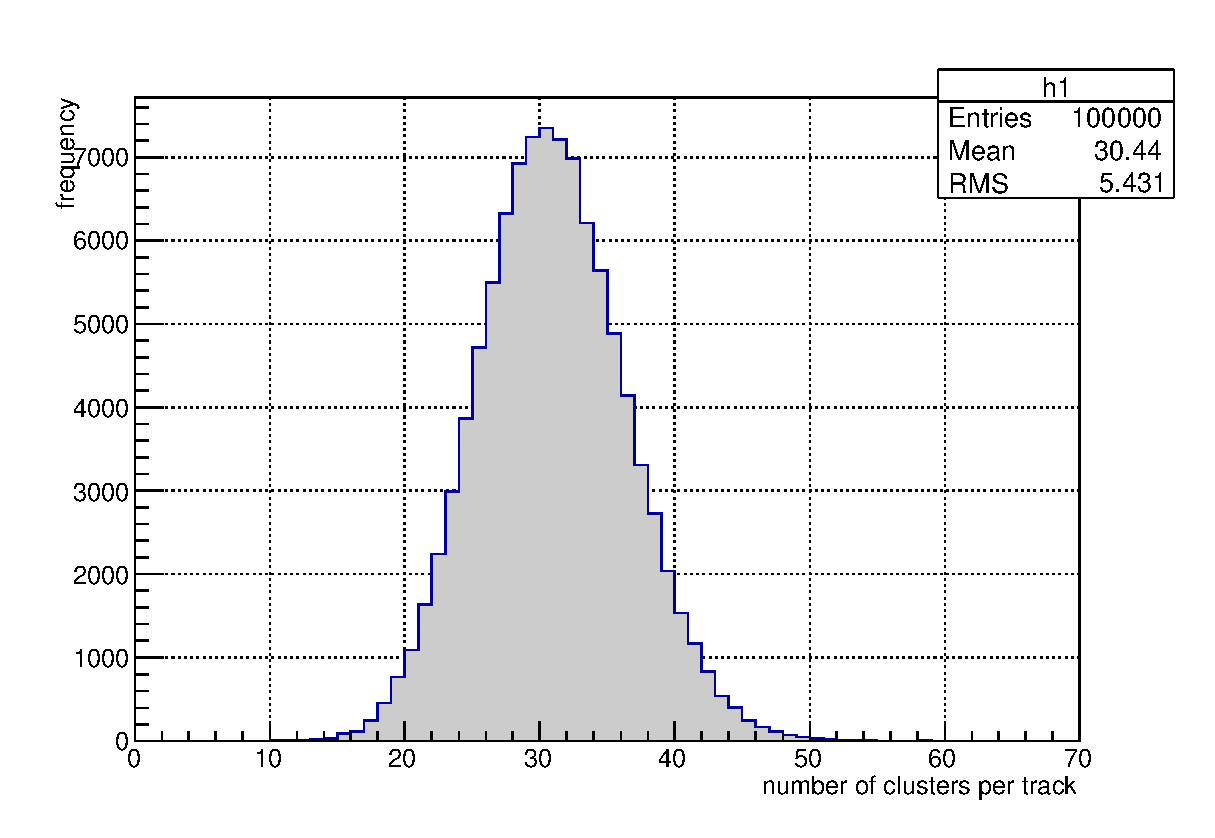
\includegraphics[width=0.45\textwidth]{cluster_distrib} 
			\label{fig:cluster_distrib} }%
			\caption{Statistics info from GARFIELD about track from $1GeV~\mu$. Tube described in table~\ref{table:straw_par}}
	\end{figure}
	
	From the Fig.\ref{fig:efficiency} we can conclude that the efficiency of tube is $100\%$ almost in whole region covered by tube except pre wall region which is quite small. Increasing the gas mixture density or increasing the tube radius for the same gas density can increase tube efficiency.